\section{Experiments}
\label{sec:diffusion_experiments}

Or main goal during this investigation into diffusion models was to get a better understanding of their performance on a wide range of tasks. We keep in mind the original task of improving an existing motion sequence, but are aware of the other potentials of the model and so do not limit ourselves in scope.


%%%%%%%%%%%%%%%%%%%%%%%%%%%%%%%%%%%%%%%%%%%%%%%%%%%%%%%%%%%%%%%%%%%%%%%%%
% General test cases
%%%%%%%%%%%%%%%%%%%%%%%%%%%%%%%%%%%%%%%%%%%%%%%%%%%%%%%%%%%%%%%%%%%%%%%%%
\subsection{Test Cases}
We present here a variety of different test cases on which the models performance can be evaluated. The general structure of the evaluation is to generate a sufficiently large number of sequences for each given task, then import them into the Blender computer graphics software and visually inspect their quality and how well they achieve each task. We have decided to take a qualitative approach as we are attempting to get a better general understanding of the models capabilities, and so this was the path of least resistance to obtain good intuition in the short time that was left after the HuMoR investigation. We note that in the future if a method is deemed worthy of further investigation, more rigorous evaluation metrics would be beneficial.

\subsubsection{Sequence Generation}
To ensure that the model has learned a sensible variety of human motion, we generate a number of sequences from Gaussian noise and check that they contain sufficient diversity, considering that a main indicator of an overfit diffusion model is that of a lack of diversity.

\subsubsection{Denoising}
\TODO{Come up with a better test for this}

\subsubsection{Occluded Legs}
An important situation in which the current Disney Research|Studious model does not perform optimally is that of occluded sequences. To test the ability of the diffusion models to handle this situation, we evaluate the models capabilities to generate the leg motion of an entire motion sequence. We achieve this using the inpainting framework described in \secref{sec:diffusion_method_inpainting}, keeping the upper body joint rotations and the root translation fixed, and allowing the model free reign over the rest of the state.

\subsubsection{Missing State}
To further test the models' ability to handle occlusions, a test case where we only keep a random percent of the state during inpainting is presented. This portion of the state to keep can either be 
\begin{enumerate}
    \item a random subset of each frame in a motion sequence
    \item a random subset that is constant across the whole sequence
\end{enumerate}
with the first testing the models' ability to handle arbitrarily occurring missing data, and the second testing the models ability to recover from longer-term occlusions.

\subsubsection{Inbetweening}
Another important area of motion generation research is that of Motion Inbetweening, in which the goal is to fill in a middle part of a motion sequence in which a number of frames at the beginning and end of the sequence are given. Again we can use the inpainting framework from \secref{sec:diffusion_method_inpainting} and keep the edges of the motion static.


%%%%%%%%%%%%%%%%%%%%%%%%%%%%%%%%%%%%%%%%%%%%%%%%%%%%%%%%%%%%%%%%%%%%%%%%%
% Baseline model
%%%%%%%%%%%%%%%%%%%%%%%%%%%%%%%%%%%%%%%%%%%%%%%%%%%%%%%%%%%%%%%%%%%%%%%%%
\subsection{Baseline Model}
\label{sec:baseline_evaluation}
The baseline model was trained with the Disney Research|Studios dataset that does not, and cannot (due to a lossy rendering of the mocap), contain foot contacts. The state includes the root translation, joint orientations, and their respective velocities explicitly.

\subsubsection{Sequence Generation}
We found that the model generates a diverse set of plausible motion, as can be seen in \figref{fig:baseline_generation}. A few shortcomings were however noted. We found that the model produces a fair bit of foot sliding, where the foot is in contact with the ground and the pose is static, but the feet have a non-zero velocity and are sliding about. This effect usually can be mitigated through the use of the foot sliding loss during training which necessitates access to data containing labeled foot contacts.

\begin{figure}[!ht]
    \centering
    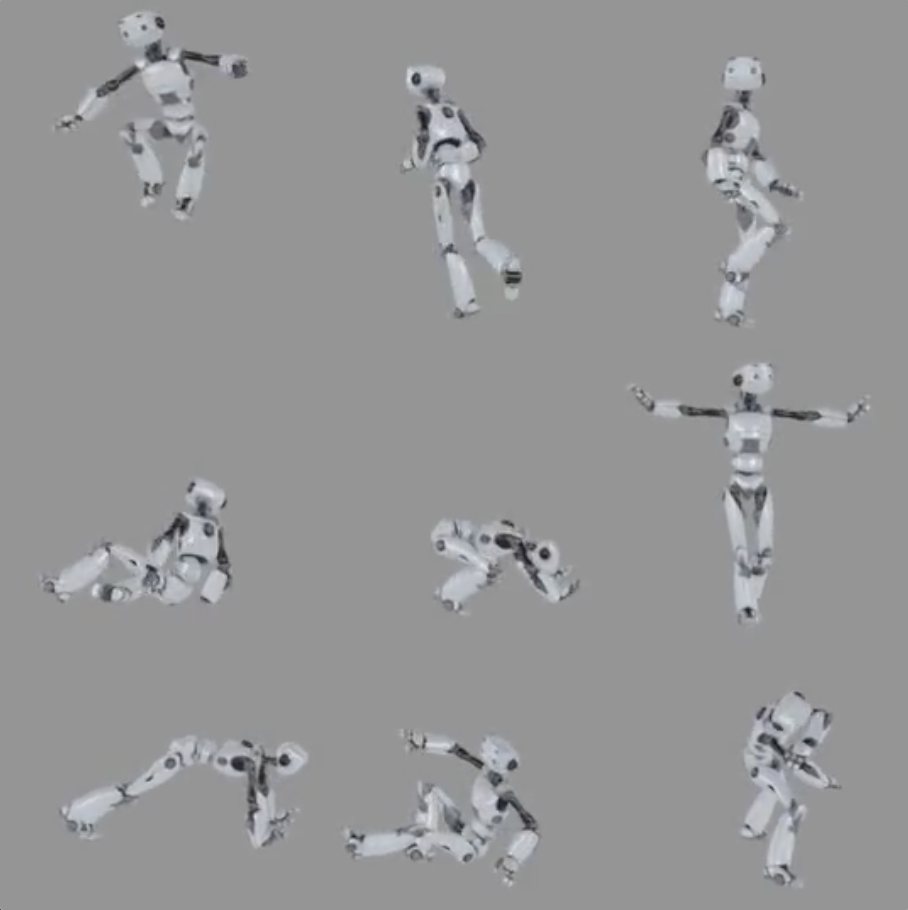
\includegraphics[width=0.75\textwidth]{Figures/diffusion/results/baseline_generation.png}
    \caption{Motion Generation - Baseline model}
    \label{fig:baseline_generation}
\end{figure}

\subsubsection{Denoising}
\TODO{Come up with a better test for this}

\subsubsection{Occluded Legs}
The model shows a strong performance on the task of inpainting missing legs in a motion sequence, with the result being of leg motion that is often both smooth and well adhering to the upper body motion. An example frame is shown in \figref{fig:baseline_occluded_legs}. 
The most notable failure case is that sometimes the model reverses the direction of motion. We postulate that this is due to the fact that the data for the baseline model has a root that does not move in the forward/reverse (x,y) direction, therefore the pendulating rotation motion of the hips, without the additional context of a specific direction, can often be both interpreted as both forward and backward walking.

\begin{figure}[!ht]
    \centering
    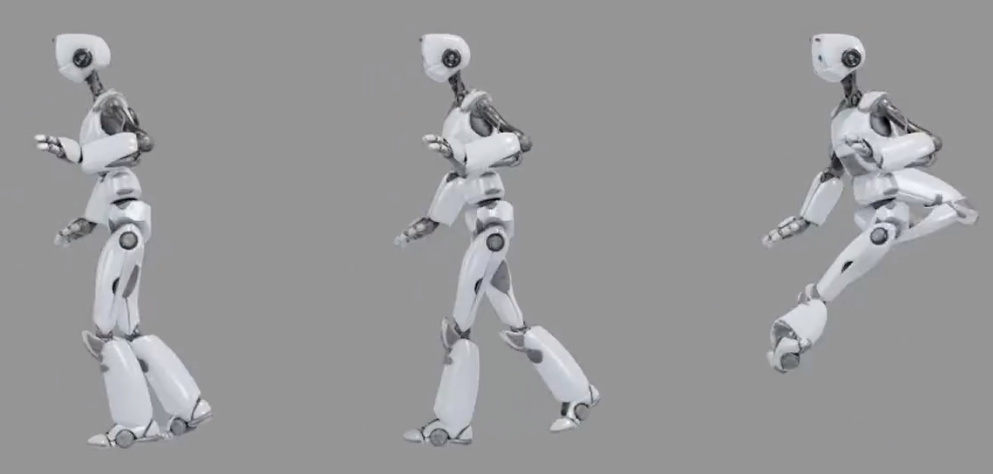
\includegraphics[width=1\textwidth]{Figures/diffusion/results/basline_inpainting_legs.png}
    \caption{Occluded Legs Inpainting - Baseline model}
    \label{fig:baseline_occluded_legs}
    \medskip
    \small
    The character on the left has the original motion, in the middle the inpaintined motion which is derived from the rightmost character, whose leg features are simply Gaussian noise
\end{figure}


\subsubsection{Missing State}
\textbf{Random each frame}
When removing a new random subset of the joints of each pose in every frame in the motion sequence, we find that the model can very accurately reconstruct the missing state, even when only 50\% of the state is given each frame, and surprisingly it still performs reasonably well when only 25\% of the state is given each frame. This shows that the model has learned well the concept of temporal consistency, as in this experiment it is likely that a missing joint will be surrounded (temporally) by known joints, hence it simply needs to interpolate between these known joints.

% \begin{figure}[!ht]
%     \centering
%     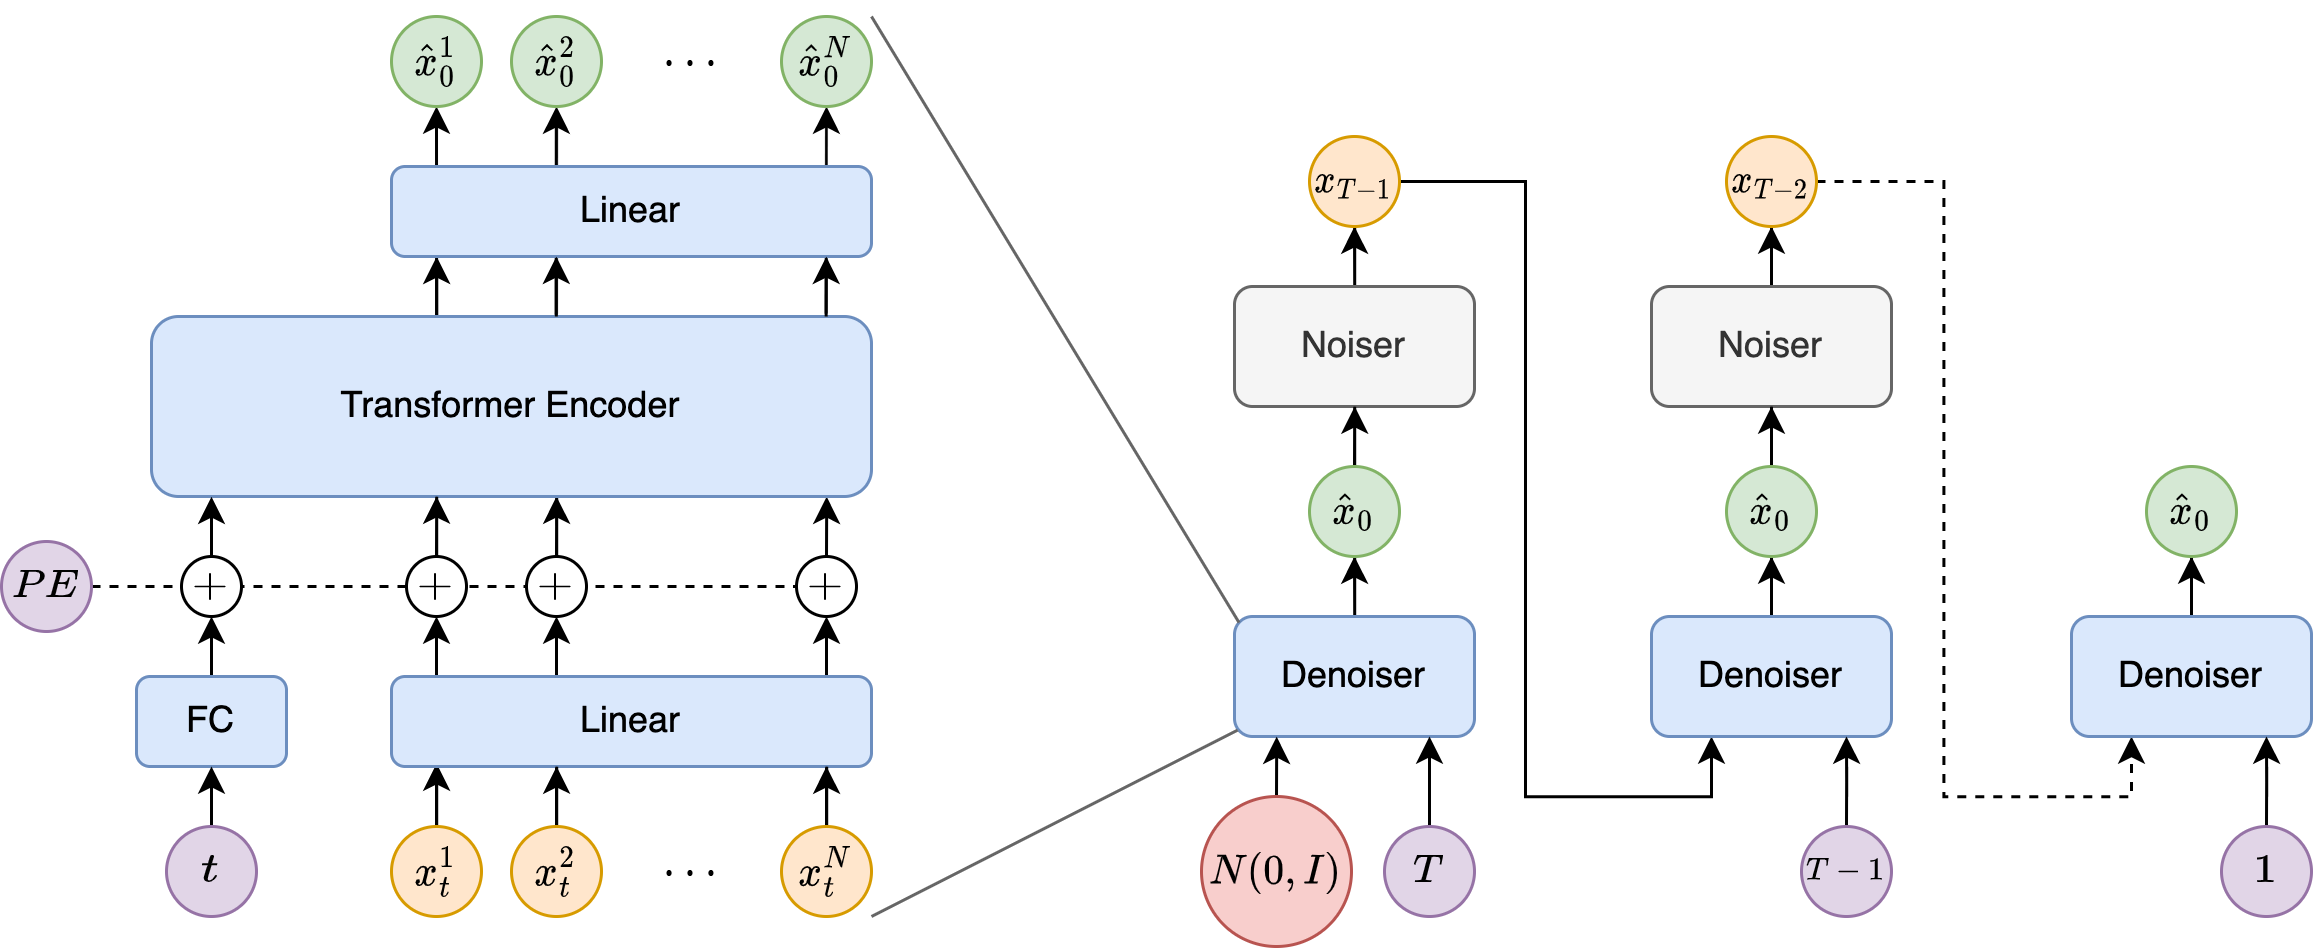
\includegraphics[width=1\textwidth]{Figures/diffusion/Network_diagram.png}
%     \caption{Occluded Legs Inpainting - Baseline model}
%     \label{fig:baseline_missing_state_random_each_frame}
% \end{figure}

\textbf{Random for the whole sequence}
\TODO{Describe the results}


\subsubsection{Inbetweening}
\label{sec:diffusion_baseline_inbetweening}

The performance on the motion inbetweening task is promising but has some flaws. The model successfully manages to interpolate between the two known motions at the extremities of the sequence and presents plausible motion in the middle, however the generated motion is not particularly related to the known motion, being oft meandering and of a different nature. Here the text conditioning of \cite{MDM} could provide benefits by restricting the possible inbetweened motion. We also note that there is a jump between the known motion and the generated motion. We investigated and found that during the final step of the denoising procedure, the last operation is that of inpainting where the known and generated motions are mixed through a binary mask. This therefore overrides the beginning and end of the generated motion with known motion. If we simply look at the generated motion, it is smooth, however, the motion that is overwritten by the known motion does not exactly match the known motion, hence the overwriting introduces a jump. This could be mitigated by using a more sophisticated inpainting method as discussed in \secref{sec:diffusion_future_work} and attempted in \secref{sec:diffusion_inbetweening_blending}.


%%%%%%%%%%%%%%%%%%%%%%%%%%%%%%%%%%%%%%%%%%%%%%%%%%%%%%%%%%%%%%%%%%%%%%%%%
% Mode with foot contacts
%%%%%%%%%%%%%%%%%%%%%%%%%%%%%%%%%%%%%%%%%%%%%%%%%%%%%%%%%%%%%%%%%%%%%%%%%
\subsection{Model with Foot Contacts - World Space}
\label{sec:diffusion_contacts_world_space}

The second model was trained in a similar manner, but with a different dataset in which the foot contact labels were given, and therefore where an extra foot contacts loss was used. We first tested this model with the motion in world space, as described in \secref{sec:diffusion_state_representation}, meaning that the start point and orientation of each motion are different. We found generally that the model still learned some reasonable motion, however that the root motion was rather disconnected from the rest of the body, resulting in foot sliding. We postulate that this is because we have now massively enlarged the state space, considering the extra dimensions of root motion added and the fact that this is unhomogenised (i.e two identical motions that start in different positions are completely distinct from the models perspective), and that combined with our limited dataset the model struggles to learn the correlation between root motion and the rest of the body.

% \subsubsection{Sequence Generation}
% \subsubsection{Denoising}
% \subsubsection{Occluded Legs}
% \subsubsection{Missing State}
% \subsubsection{Inbetweening}

% %%%%%%%%%%%%%%%%%%%%%%%%%%%%%%%%%%%%%%%%%%%%%%%%%%%%%%%%%%%%%%%%%%%%%%%%%
% % Mode with foot contacts
% %%%%%%%%%%%%%%%%%%%%%%%%%%%%%%%%%%%%%%%%%%%%%%%%%%%%%%%%%%%%%%%%%%%%%%%%%
% \subsection{Model with Foot Contacts - 'Stuck' Space}

% To overcome the issue of \secref{sec:diffusion_contacts_world_space} we aligned all the motion to begin at the same point and facing the same direction. The results are that...
% \TODO{Finish debugging then conclude here}

%%%%%%%%%%%%%%%%%%%%%%%%%%%%%%%%%%%%%%%%%%%%%%%%%%%%%%%%%%%%%%%%%%%%%%%%%
% Autocompletion
%%%%%%%%%%%%%%%%%%%%%%%%%%%%%%%%%%%%%%%%%%%%%%%%%%%%%%%%%%%%%%%%%%%%%%%%%
\subsection{Autocompletion}
\label{sec:autocomplete}

Another project that is running at Disney Research|Studios is that of pose autocompletion. This is the task of taking a set of \textit{handles}, a subset of joints, and predicting the position of the rest of the joints. The goal here is again to help to improve the animation pipeline, this time by reducing the amount of work an animator has to do to get a sensible pose. As a side note to the previous experiments to understand the generality of these diffusion models, we trained some diffusion models for the described task, where we enforce a sequence length of 1 so that we are only predicting a single pose, and where we modify the inpainting to allow for a specific set of joints to be deemed \textit{handles} and to be kept fixed.

\subsubsection{Baseline}
The model is as described in \secref{sec:baseline_evaluation} however with a sequence length of 1.

We find that while the model does present plausible poses, and that on average these poses have handle joints close to the desired positions of the handles (with a few exceptions), it does not satisfy the task properly.  An ideal solution would not move the handles at all, and would simply modify the rest of the joints.

%  as can be seen in \TODO{include images of position of handles vs. position of actual joints}.
% \TODO{include images}


\subsubsection{Handle Conditioning}
To mitigate this issue of the handles being modified, we propose handles conditioning, in which a one hot embedding of the handles is run through a linear layer, then concatenated to the input of the network. A loss is then applied to the output that penalises any deviation in the position of the handles that are output as compared to those input. In theory, this should force the network to learn to consider the handles as immutable and to create a pose that satisfies the handles.

Though the implementation was largely completed, we unfortunately did not have time to finish debugging some of the finer details, so cannot provide concrete results. However we deemed the idea interesting enough to present in this thesis, and hope that it can be of use in future research.


\subsection{Other Experiments}
\subsubsection{Denoising steps}
One drawback of diffusion models is that the denoising procedure is iterative, that is to say if we train with 1000 denoising steps, we then denoise with the same number of steps. Thus, while it is a direct prediction model unlike the optimisation procedure presented in \chpref{chpt:humor}, it still does not provide immediate results. Various strategies have been presented to mitigate this issue. A notably succesful strategy for speeding up the denoising procedure for image generation is that of diffusing in some latent encoding space \cite{stable_diffusion}, thereby reducing the dimensionality of the state that the denoising model operates on. Another strategy, presented in \cite{improved_diffusion}, is simply denoising with less steps. In essence rather than denoising from step 1000 -> 999 -> 998 -> ... you stride the denoising procedure, 1000 -> 950 -> 900 -> ... which only requires a reweighting of the noise schedule. 

We tested this latter strategy on our model, denoising with various numbers of steps. We found that denoising with anything down to 100 steps provided visually identical results to denoising with 100 steps, however, below, with 10 steps for example, the quality of the motion deteriorates. This is an exciting result as it suggests that we can achieve interesting results in a reasonable amount of time, thereby indicating that such a model could be employed in production and provide users with results within an acceptable time frame.

\subsubsection{Inbetweening Blending}
\label{sec:diffusion_inbetweening_blending}

In \secref{sec:diffusion_baseline_inbetweening} we noted a discontinuity between the known motion and the generated motion. We hypothesised that this was due to the inpainting procedure, and that a more sophisticated inpainting procedure could mitigate this issue. We therefore implemented a denoising procedure in which pad the edges of the known regions of motion with the last known pose, and rather than using a binary mask, we blend this padded region with the generated motion smoothly. With this procedure we aim at forcing the model to generate a motion that is continuous with the known motion. We find that this procedure, when coupled with the model operating on motion with freely moving root presented in \secref{sec:diffusion_contacts_world_space}, looks rather like a simple linear interpolation between the two motion. We postulate that this is due to the shortcoming of the model, notably that the root motion is not well learned and so is often very far from the known root motion. However, for the model operating on motion with fixed root presented in \secref{sec:baseline_evaluation}, we find that \TODO{Test this, hopefully is nice}.